\chapter{Emergence of Object-level Information in Deep Networks}

\todo{To be written.}

%With the previous chapters showing the effectiveness of feature learning and concept learning in a more ``conventional'' pipeline that employs separately designed, modular components, we 

%As the vision community has only recently rediscovered the power of deep convolutional neural networks, much remains to be analyzed and understood. Thus, compared to previous ones, this chapter is presented in a more exploratory and empirical way, in the hope that it will shed lights guidance for future research on this groundbreaking direction.


\section{Background}
Discovery of effective representations that capture salient semantics
for a given task is a key goal of perceptual learning.  Performance
with conventional visual representations, based on flat feature
representations involving quantized gradient filters, has been
impressive but has likely plateaued in recent years.

It has long been argued that deep or layered compositional
architectures should be able to capture salient aspects of a given
domain through discovery of salient clusters, parts, mid-level
features, and/or hidden units
\cite{autoencoders,fidler,yuille2007,efros2012,supervision}. Such models have
been able to perform better than traditional hand-engineered
representations in many domains, especially those where good features
have not already been engineered \cite{ngunsupervised}.  Recent
results have shown that moderately deep unsupervised models outperform
the state-of-the art gradient histogram features in part-based
detection models \cite{hsc}. However, unsupervised deep models with
more than a few layers have proven difficult to train on large-scale visual category recognition tasks.

Deep models have recently been applied to large-scale
visual recognition tasks, trained via back-propagation through layers of convolutional filters
\cite{lecun89}. These models perform extremely well in domains with
large amounts of training data, and had early success in digit
classification tasks \cite{lenet}. With the advent of large scale
sources of category-level training data, e.g., \cite{imagenet_cvpr09}, and
efficient implementation with on-line approximate model averaging
(``dropout'') \cite{supervision}, they have recently outperformed all
known methods on a large scale recognition challenge
\cite{ilsvrc2012}.

%Deep convolutional networks have a long history in computer vision, with early examples showing successful results on using supervised back-propagation networks to perform digit recognition~\cite{lecun89}.
%More recently, these networks, in particular the convolutional network proposed by~\cite{supervision}, have achieved competition-winning numbers on large benchmark datasets consisting of more than one million images, such as ImageNet~\cite{ilsvrc2012}.

With limited training data, however, fully-supervised deep
architectures with the representational capacity of \cite{supervision}
will generally dramatically overfit the training data.
In fact, many conventional visual recognition challenges have tasks with few
training examples; e.g., when a user is defining a category
``on-the-fly'' using specific examples, or for fine-grained
recognition challenges \cite{birds}, attributes \cite{attribute}, and/or
domain adaptation \cite{eccv_saenko}.

Learning from related tasks also has a long history in machine learning beginning with~\cite{caruana1997multitask} and~\cite{thrun1996learning}. Later works such as~\cite{argyriou2008convex} developed efficient frameworks for optimizing representations from related tasks, and~\cite{ando2005framework} explored how to transfer parameter manifolds to new tasks. In computer vision, forming a representation based on sets of trained classifiers on related tasks has recently been shown to be effective in a variety of retrieval and classification settings, specifically using classifiers based on visual category detectors~\cite{torresani2010efficient,li2010object}. A key question for such learning problems is to find a feature representation that captures the object category related information while discarding noise irrelevant to object category information such as illumination.

Transfer  learning across tasks using deep representations has been extensively studied, especially in an unsupervised setting~\cite{raina2007self,mesnil2012unsupervised}. However, reported successes with such models in convolutional networks have been limited to relatively small datasets such as CIFAR and MNIST, and efforts on larger datasets have had only modest success~\cite{googlebrain}.  We investigate the ``supervised pre-training'' approach proven successful in computer vision and multimedia settings using a concept-bank paradigm \cite{lscom,li2010object,torresani2010efficient} by learning the features on large-scale data in a supervised setting, then transferring them to different tasks with different labels.

To evaluate the generality of a representation formed from a deep convolutional feature trained on generic recognition tasks, we consider training and testing on datasets known to have a degree of dataset bias with respect to ImageNet. We evaluate on the SUN-397 scene dataset, as well as datasets used to evaluate domain adaptation performance directly~\cite{ref:dlid,ref:kulis_cvpr11}. This evaluates whether the learned features could undo the domain bias by capturing the real semantic information instead of overfitting to domain-specific appearances.

\section{Caffe: A Convolutional Architecture for Fast Feature Embedding}
While deep convolutional features have gained much interest in the literature, there exists little, if any, toolboxes that provides a truly off-the-shelf deployment of state-of-the-art models, and it is often nontrivial to replicate experimental results reported in the recent papers without involving substantial graduate student time. To facilitate the wide-spread need for deep convolutional features and analysis, I developed a C++ framework that allows one to efficiently experiment with such architectures. I will elaborate a few key system design choices below, and the reader is encouraged to read more technical details on the Caffe website at \url{http://caffe.berkeleyvision.org/}.

\subsection{Key Design Choices}
\paragraph{GPUs: Necessary for Training} With the large computation needs like the convolutional neural networks have, it is virtually impossible to train networks with CPU only. While systems such as the Google Brain \cite{le2012icml} is able to address this by leveraging thousands of machines, the budget for such systems may be overly prohibitive. Thus, I depend highly on GPUs to perform computation, with specific care to hide implementation details from researchers who use them.

I used the Nvidia K20 GPU to perform all experiments mentioned in this work, but note that in terms of vision applications, strict scientific computing features such as ECC do not appear to be significant, and commodity GPUs, such as GTX780, works as well with no noticeable performance difference.

\paragraph{Data Storage} With the high throughput of GPUs, it is important that one selects a highly efficient data storage to load data from. For example, laying images on disk and randomly reading them leads to a disk throughput of about 6M/s, while the GPU usually requires about 30M/s data throughput\footnote{Measured when using the SuperVision model by Krizhevsky et al.}. Thus, I chose to store data in the LevelDB database \footnote{https://code.google.com/p/leveldb/} with the Google ProtoBuffer format \footnote{https://code.google.com/p/protobuf/}. When combined together, they provide about 150M/s throughput with commodity hard disks (not solid state drives), allowing one to efficiently utilize the full computation capability of GPUs.

\paragraph{Segregation of Interface and Implementation} While GPU provides an efficient way to carry out computation, managing GPU codes are known to be difficult especially for highly customized code. Thus, we designed the system with a clear segregation of the interface from specific implementations. Specifically, we proposed a general wrapper that manages synchronized CPU and GPU memories, and all operations are defined on the wrapper. As a result, one is able to define the network without having to specify which architecture it uses. During runtime, depending on whether the user runs with a GPU or not, the code would seamlessly switch between CPU and GPU code, without the need of user intervention or any reimplementation. The synchronized wrapper also provided possibility to extend to further platforms, such as mobile, as the network is explicitly defined in a device-independent way.


\paragraph{CPUs: Still Hope} It is worth noting that while training may be difficult with CPUs, inference is still very affordable with them. In practice, the Caffe CPU implementation is able to run the ImageNet SuperVision model at a speed of 20 milliseconds per frame on a state-of-the-art CPU (with 8 cores) when images are provided in minibatches. This actually allows almost real-time computation, and is valuable since most existing computation architectures may not have GPUs yet.

\paragraph{Implementation of Convolution} To perform convolution in an efficient way, we chose a path that is memory heavy: each local patch is expanded to a separate vector, and the whole image is converted to a matrix whose rows correspond to the multiple locations where filters will be applied. This effectively converts the convolution to a matrix-matrix multiplication ({\texttt gemm}) call, making it possible to utilize the commonly available, highly optimized BLAS (CUBLAS on Nvidia GPUs) libraries for dense computation.

While one may question the speed of such operations, we note that the most time-consuming part of convolution is the dense {\texttt gemm}. Assuming we have an image of size $N\times N$, a filter size of $K\times K$ and a total number of 
$F$ filters, then the matrix expansion mentioned above will only account for $O(N^2K^2)$ complexity while the matrix multiplication complexity is $O(N^2K^2F)$. In the case of deep networks, F is usually very large (e.g.\ 256), effectively amortizing the expansion overhead. In practice, we observed a speedup of about 1.3 times on K20 compared to cuda-convnet\footnote{\url{https://code.google.com/p/cuda-convnet/}}, which is optimized for GTX580.

\paragraph{Notes on Multi-GPU computation} The current Caffe implementation does not utilize multiple GPUs, but as a general note, it is possible that multiple GPUs on the same machine could be used for faster computation - effectively, one may distribute the minibatches during training to different GPUs in an asynchronous fashion. Combining different GPUs on different machines may be more complex, as there are multiple latency issues (such as the network latency) that needs to be accounted for. Related work such as \cite{coates2013deep} have shown promising results with custom, fast networks, and may be a valuable engineering direction to pursuit in the future.

\subsection{Training Details}
As the underlying architecture for higher-level analysis, I adopted the deep convolutional neural network architecture proposed by Krizhevsky \etal \cite{krizhevsky2012imagenet}, which won the ImageNet Large Scale Visual Recognition Challenge 2012 with a top-1 validation error rate of 40.7\%\footnote{The model entered into the competition actually achieved a
top-1 validation error rate of 36.7\% by averaging the predictions
of 7 structurally identical models that were initialized and trained
independently. We trained only a single instance of the model;
hence we refer to the single model error rate of 40.7\%.
}. This model is chosen due to its performance on a difficult 1000-way classification task, hypothesizing that the activations of the neurons in its late hidden layers may serve as very strong features for a variety of object recognition tasks. Its inputs are the mean-centered raw RGB pixel intensity values. These values are forward propagated through five convolutional layers (with pooling and ReLU non-linearities applied after certain convolutional layers) and three fully-connected layers to determine its final neuron activities: a distribution over the task's 1000 object categories.

I refer to the original paper for a detailed discussion of the architecture and training protocol, which we closely followed with the exception of a few small differences in the input data: (1) I ignored the images' original aspect ratio and warp them to $256\times 256$, rather than resizing and cropping to preserve the proportions; (2) Images are cropped to $227\times 227$ rather than $224\times 224$ as in the original paper, due to the difference in the convolutional layers' implementations; (3) I did not perform data augmentation by adding random multiples of the principle components of the RGB pixel values throughout the dataset, which was used as a way of capturing invariance to changes in illumination and color. For training, 90 epochs through the data are carried out, with an initial learning rate of 0.01 and dropped by a factor of 10 after epochs 25, 50, and 75.

The model, when trained with Caffe, took about 6 days to converge on a single K20 GPU. the final model achieved a top-1 error of 41.7\%, which is 1\% shy of the performance reported in \cite{krizhevsky2012imagenet}. According to the authors, the data augmentation accounts for about 1\% performance difference, which explains most of the networks' performance discrepancy.

\section{Time Analysis}
It is of particular interest to analyze the time distribution over different layers, and over different computation architectures. In our earlier publication \cite{donahue2013decaf}, we presented a preliminary analysis of per-layer speed distributions\footnote{In all experiments below, I will omit the data layer, whose speed is largely dependent on hardware such as hard disk read speed, and is of less interest.}. In this section, I will provide a more complete analysis, which hopefully provides more insights into further optimization of the learned networks.

I first compare the computation time of both the forward and backward pass, on both GPUs and CPUs, using a batch size of 256 which is typical during training time. Table \ref{table:caffe:time} summarizes the computation time of each component. In general, using a GPU speeds computation by about 10 times, both in the forward and the backward pass. Considering the fact that training the ImageNet takes about a week as also independently reported by multiple research papers, GPUs do serve as a more cost-effective solution, especially considering the fact that computation could be further speeded up with multiple GPUs on the same computer.

\begin{table}
  \centering
  \begin{tabular}{c|cc}
    \hline
    Architecture & Forward Pass & Backward Pass\\
    \hline
    GPU & 2.38 & 4.42 \\
    CPU & 28.76 & 54.99 \\
    \hline
  \end{tabular}
  \caption{The computation time of both the forward and backward pass, on both GPUs and CPUs, using a batch size of 256. The computation time reported is on each image in milliseconds, averaged over 10 independent batches.}\label{table:caffe:time}
\end{table}

\begin{figure}
  \centering
  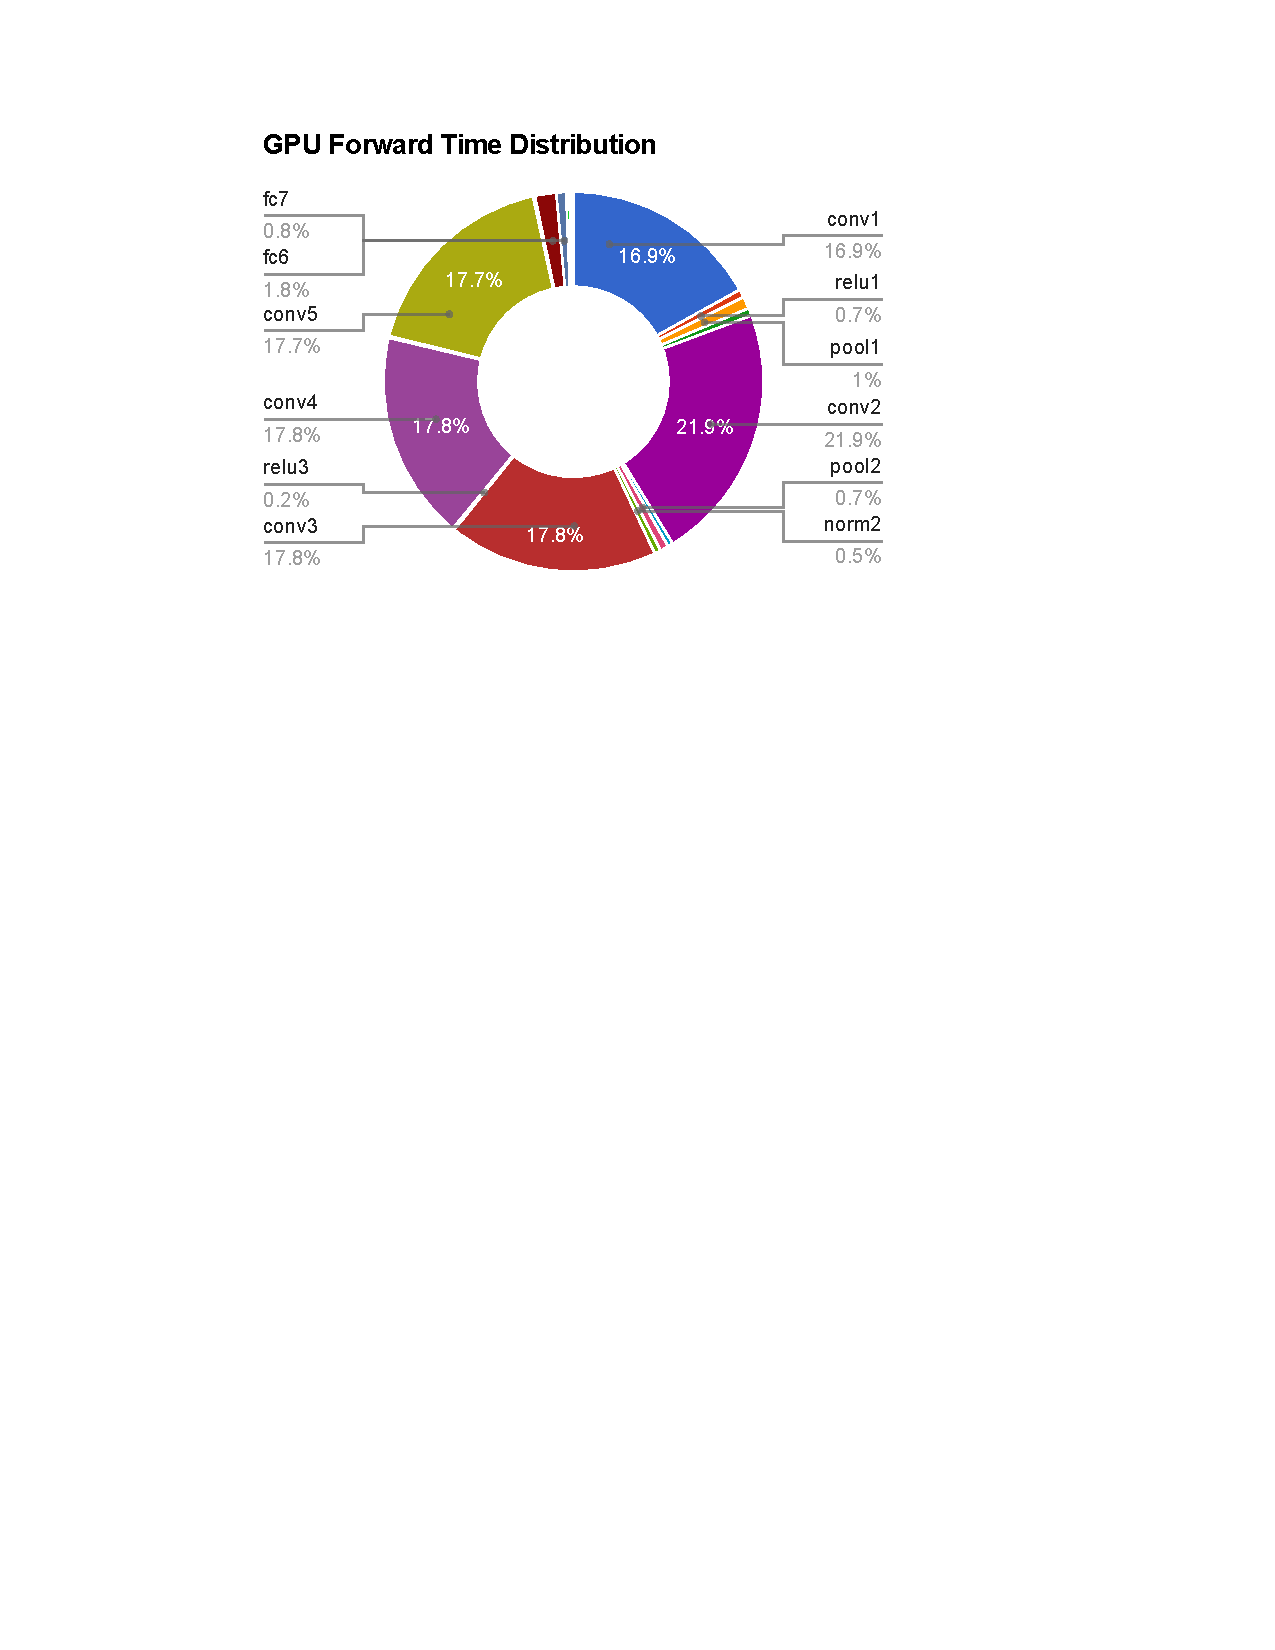
\includegraphics[width=0.45\textwidth]{figs/caffe/gpu_forward_distribution.pdf}%
  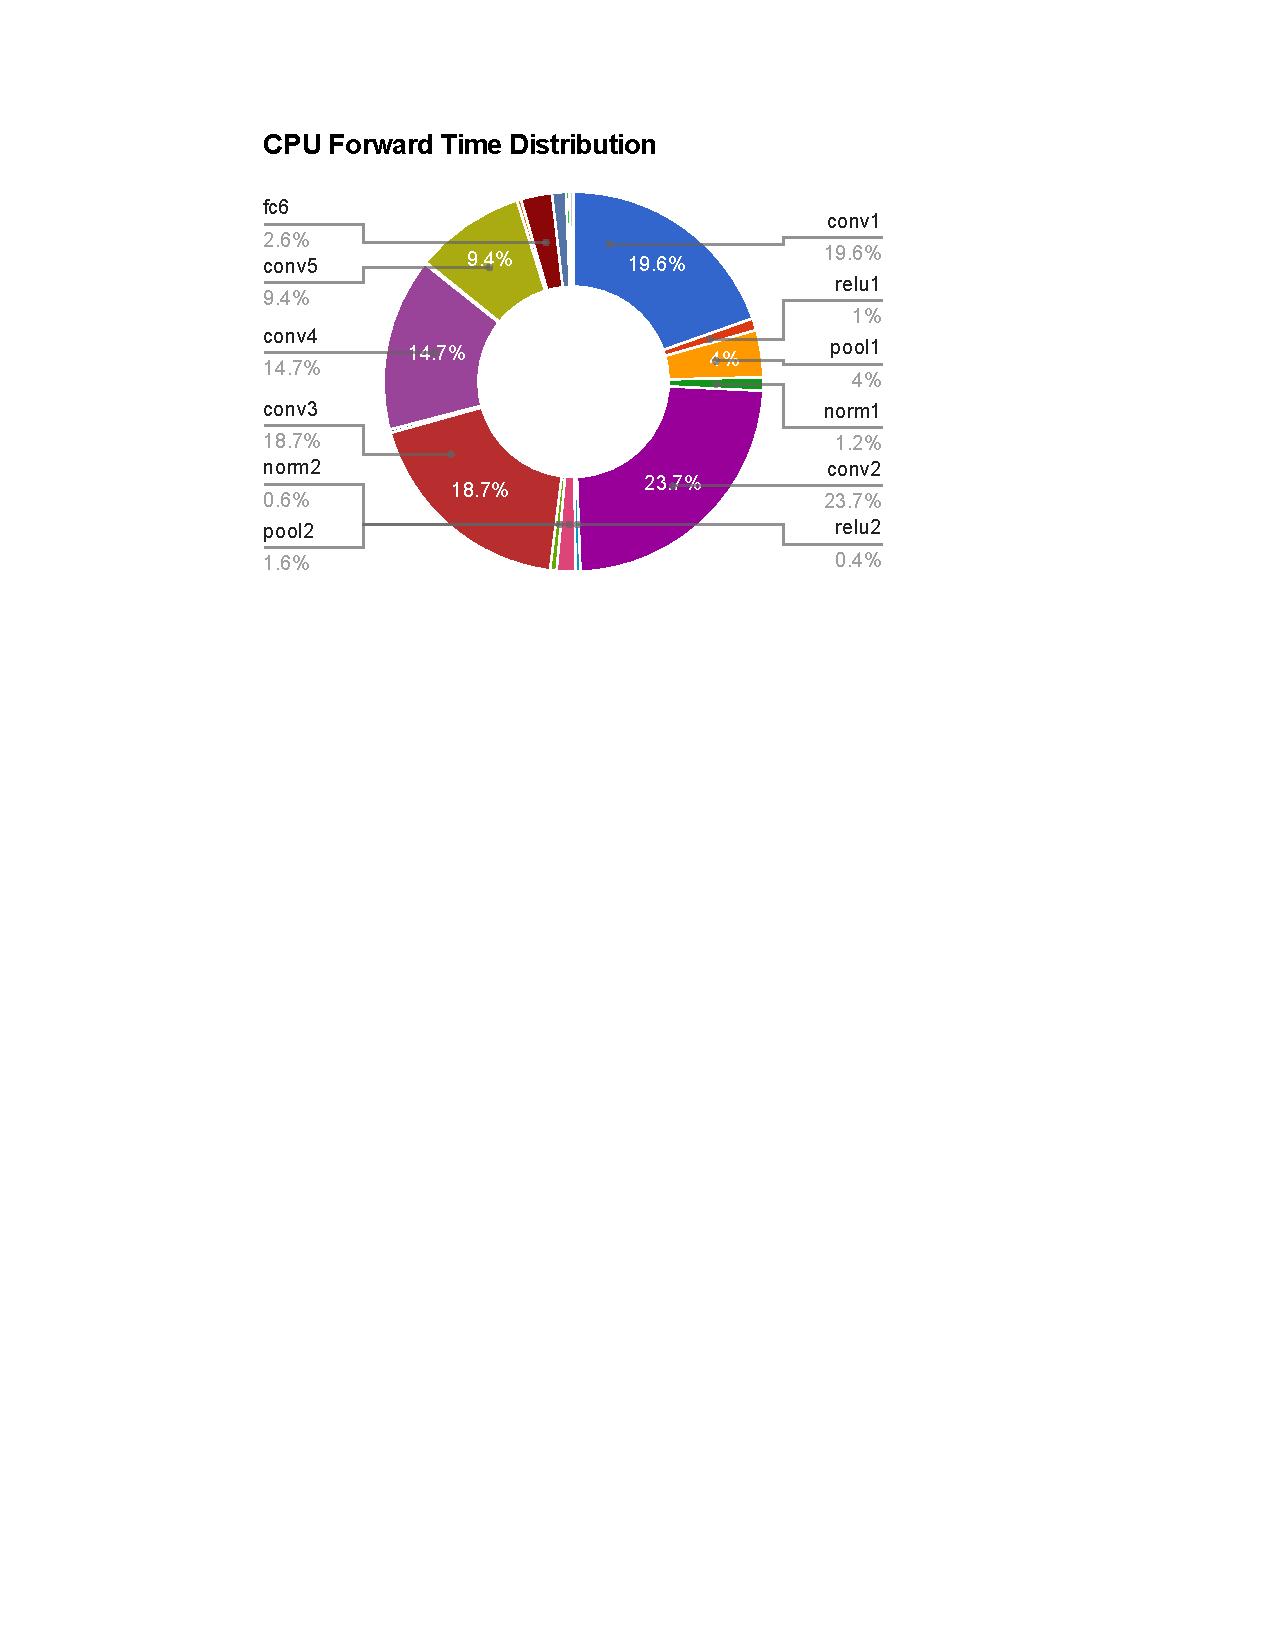
\includegraphics[width=0.45\textwidth]{figs/caffe/cpu_forward_distribution.pdf}
  \caption{Computation time distribution of individual layers, on both GPUs and CPUs for the forward pass.}\label{fig:caffe:perlayer}
\end{figure}

Further, Figure \ref{fig:caffe:perlayer} shows the computation time distribution of individual layers on both GPUs and CPUs for the forward pass. The backward pass distribution is similar so they are omitted here. It could be observed that both platforms spend most computation time on dense convolution and fully connected layers, but the GPU is better capable of handling layers that are memory-bounded, such as pooling and normalization, possibly due to the high memory bandwidth inside the GPU.

It is usually the case that computation is carried out in minibatches. This comes due to 2 reasons: (a) the stochastic gradient descent itself has been shown to work well with minibatches, and (b) minibatches usually amortizes certain computation such as converting matrix-vector multiplication to matrix-matrix multiplication, making computation more efficient than single inputs.

To analyze how the batch size affects the overall computation time, I will use the forward pass only with the GPU computation, and vary the batch size from 1 to 256, which is the range one usually chooses batch sizes from. The absolute time spent by each layer per image is shown in Figure \ref{fig:caffe:batchtime}. Note that we only visualize the eight most time-consuming layers, and omit computationally inexpensive layers such as pooling and ReLU. In total, the rest of the layers takes less than 5\% of the total computation time (see Figure \ref{fig:caffe:batchtime})

\begin{figure}
  \centering
  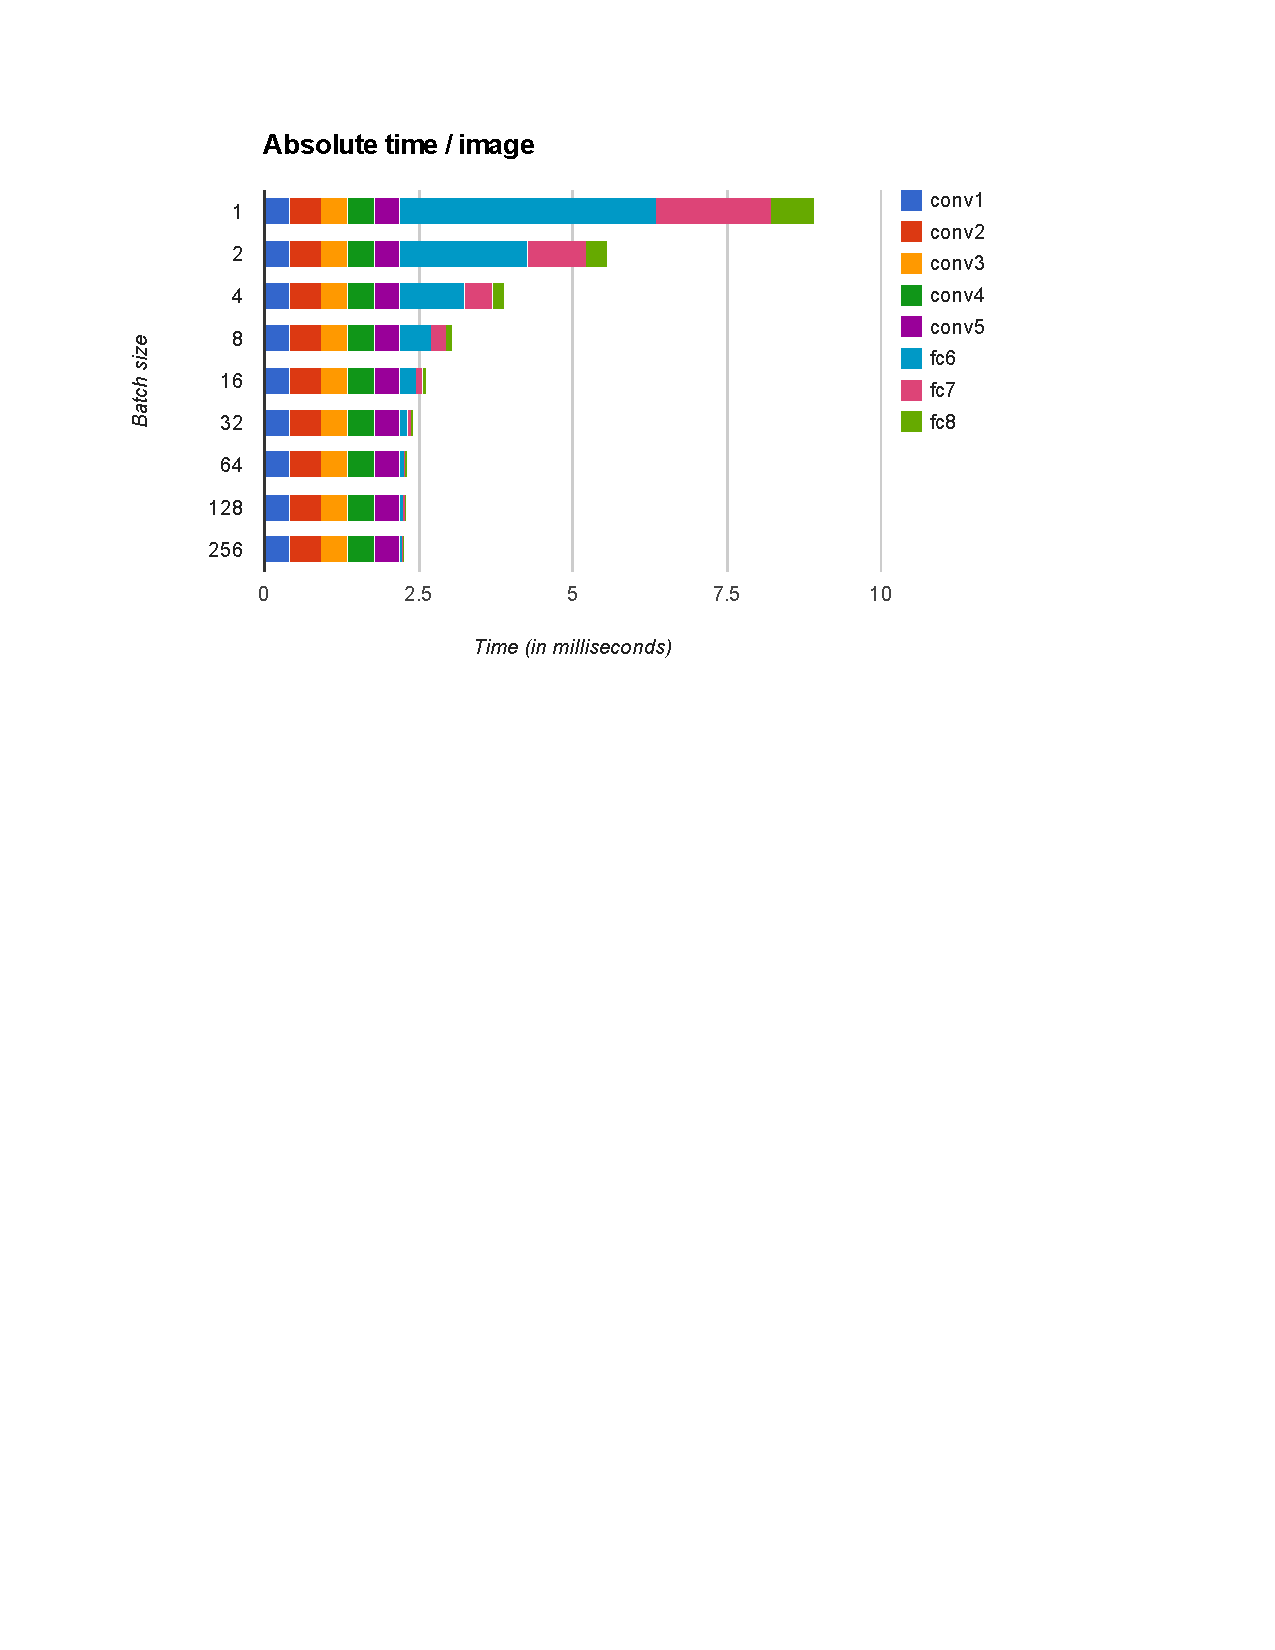
\includegraphics[width=0.8\textwidth]{figs/caffe/caffe_batchtime.pdf}\\
  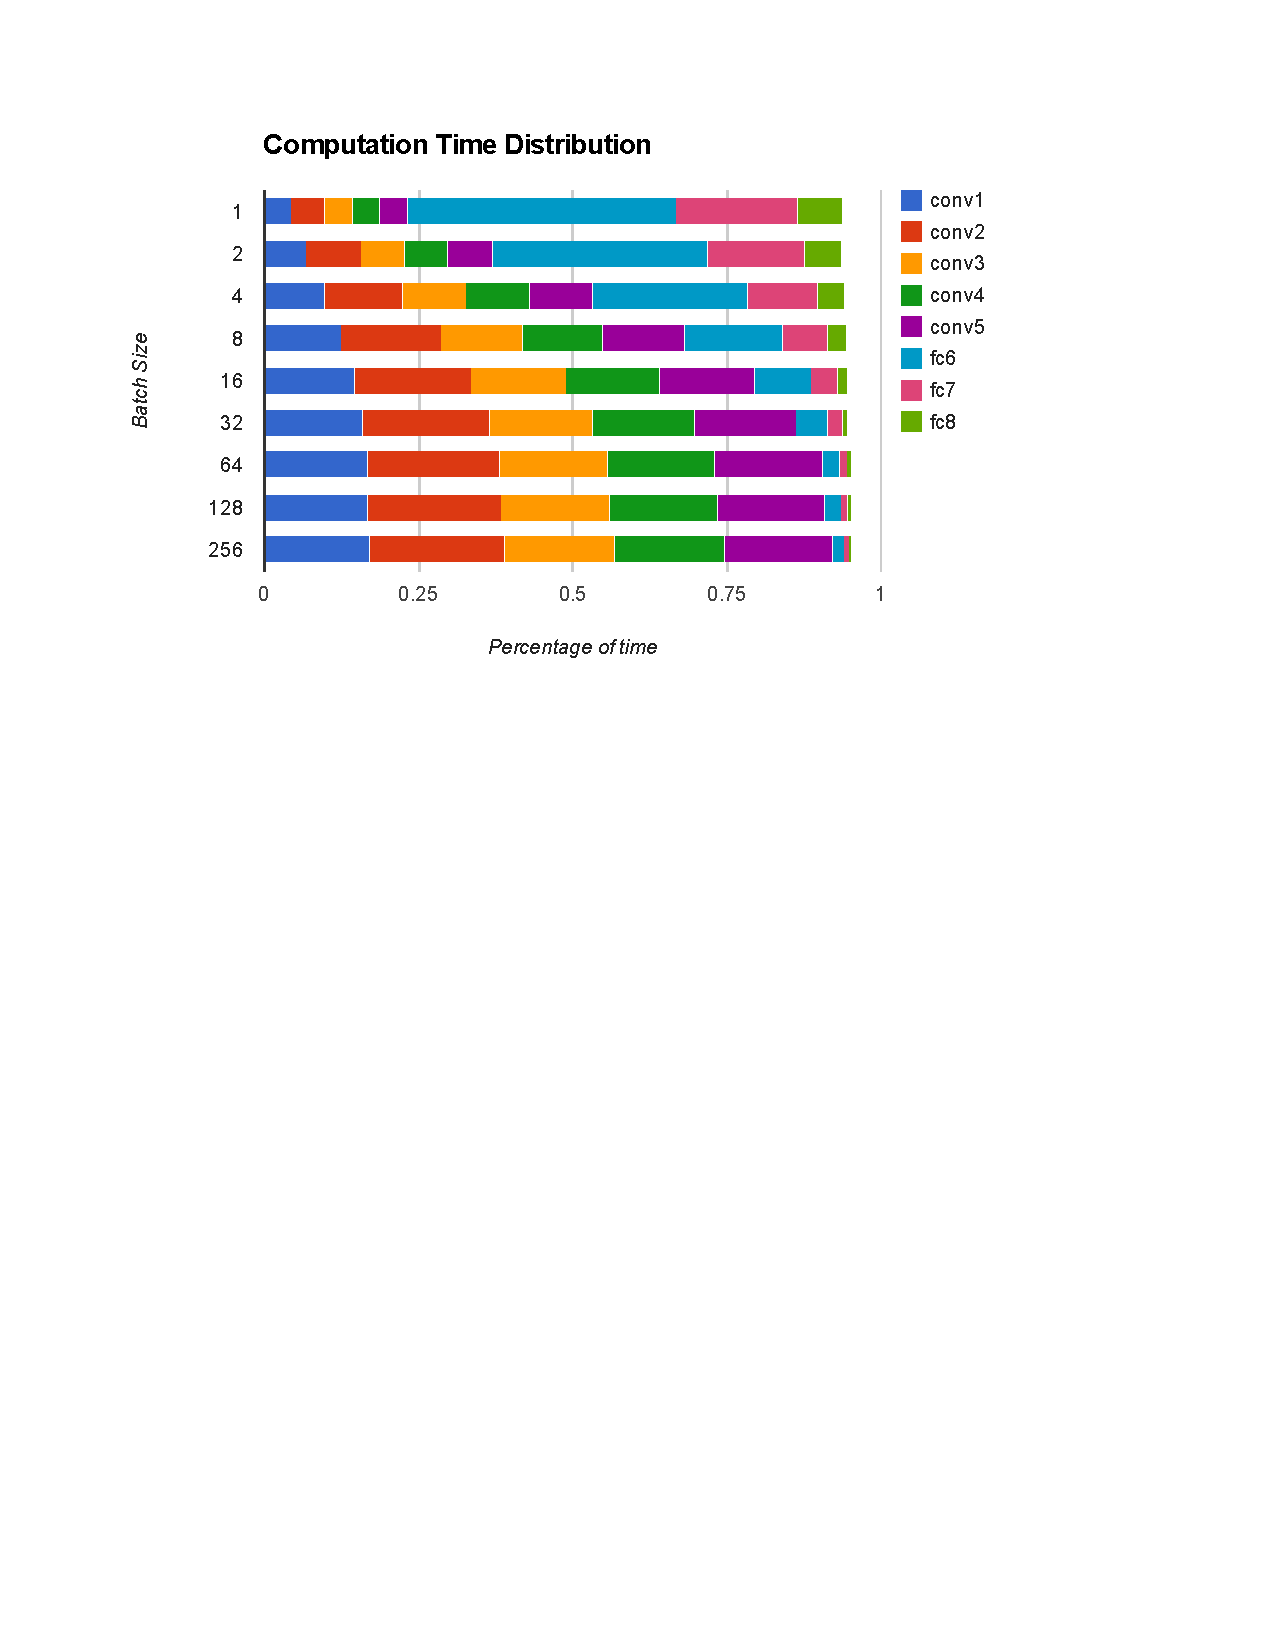
\includegraphics[width=0.8\textwidth]{figs/caffe/caffe_batchtime_relative.pdf}
  \caption{Top: absolute computation time spent on each layer per image, when the batch size varies from 1 to 256. Bottom: an alternative view of the top chart, showing the relative percentage of computation time by each layer. Note that in both figures, low-cost layers such as pooling and ReLU are not shown, which accounts for the 5\% unoccupied percentage in the bottom figure.}\label{fig:caffe:batchtime}
\end{figure}

Similar to what have been shown in \cite{donahue2013decaf}, when single images are fed into the network, the fully-connected layers takes most computation time, almost three times as expensive as the convolution layers. However, with minibatches, the computation time of the fully connected layers are quickly amortized, eventually only accounting for less than 5\% of the total computation time.

Based on the results in the two subsections above, I make the following notes:
\begin{enumerate}
  \item In a deployed system such as an online API or a video processing application, one may group requests in batches (such as aggregating multiple frames) to more efficiently use the computation resource.
  \item When single-image processing is a must, optimization on the fully connected layers are necessary, especially to reduce the number of hidden units. It is worth pointing out that the \nystrom sampling perspective I discussed in earlier chapters may be particularly helpful in this case.
  \item Convolutional layers, even when carried out with single images, is already efficient enough. At some level, this contradicts with common belief that minibatches have to be used for efficient computation. As a result, it is possible to use convolutional layers on a very large image with little loss of efficiency.
  \item While most existing detection approaches attack the detection problem in a separately designed paradigm, which first finds bounding box proposals with low-level cues and then perform classification on each bounding box, the efficiency of convolutional layers makes it applicable to perform detection in a sliding window fashion. Note that in detection, the fully-connected layers could be trivially converted to convolutional layers, making the whole pipeline highly efficient.
\end{enumerate}

\section{On the Effectiveness of Feature Transfer}
Since the network is trained with a large number of images and a large number of classes, a reasonable conjecture is that intermediate representations in this network will be useful as a general-purpose feature that performs well on related tasks, in a feature transfer fashion. In this section, a systematic examination is carried out to verify to what extent such conjecture holds.

Specifically, we present experimental results on multiple standard computer vision benchmarks, comparing many possible featurization and classification approaches.
In each of the experiments, we take the activations of the $n^{\mathrm{th}}$ hidden layer of the deep convolutional neural network described in the previous section as a feature. The following layers are used for evaluation:
(1) FC$_7$, which denotes features taken from the final hidden layer -- i.e., just before propagating through the final fully connected layer to produce the class predictions; (2) FC$_6$, which is the activations of the layer before FC$_7$, and (3) POOL$_5$, which is the last set of activations that has been fully propagated through the convolutional layers of the network.
We chose not to evaluate features from any earlier in the network, as the earlier convolutional layers are unlikely to contain a richer semantic representation than the later features which form higher-level hypotheses from the low to mid-level local information in the activations of the convolutional layers.
Because we are investigating the use of the network's hidden layer activations as features, all of its weights are frozen to those learned on the ILSVRC2012 dataset.\footnote{We also experimented with the equivalent feature using randomized weights and found it to have performance comparable to traditional hand-designed features.}
All images are preprocessed using the procedure described for the ILSVRC images in Section~\ref{sec:decaf}, taking features on the center $227 \times 227$ crop of the $256 \times 256$ resized image.

We present results on multiple datasets to evaluate the strength of DeCAF for basic object recognition, domain adaptation, fine-grained recognition, and scene recognition. These tasks each differ somewhat from that for which the architecture was trained, together representing much of the contemporary visual recognition spectrum.

\subsection{General Object Recognition}\label{sec:caltech}
To analyze the ability of the deep features to transfer to basic-level object category recognition, we evaluate them on the Caltech-101 dataset~\cite{caltech101}.
In addition to directly evaluating linear classifier performance on FC$_6$ and FC$_7$, we also report results using the dropout regularization technique proposed by~\cite{hintondropout}, which is also present in the Imagenet training phase.
At training time, this technique works by randomly setting half of the activations (here, our features) in a given layer to 0.
At test time, all activations are multiplied by 0.5.
Dropout was used successfully by~\cite{krizhevsky2012imagenet} in layers 6 and 7 of their network; hence we study the effect of the technique when applied to the features derived from these layers.

In each evaluation, the classifier, a logistic regression (LogReg) or support vector machine (SVM), is trained on a random set of 30 samples per class (including the background class), and tested on the rest of the data, with parameters cross-validated for each split on a 25 train/5 validation sub-split of the training data.
The results in Table \ref{tab:caltech101results} are reported in terms of mean accuracy per category averaged over five data splits.

\begin{table}
\centering
\begin{tabular}{lccc}
\hline
& POOL$_5$ & FC$_6$ & FC$_7$ \\
\hline
LogReg & $63.29 \pm 6.6$ & $84.30 \pm 1.6$ & $84.87 \pm 0.6$ \\
LogReg with Dropout & - & $86.08 \pm 0.8$ & $85.68 \pm 0.6$ \\
SVM & $77.12 \pm 1.1$ & $84.77 \pm 1.2$ & $83.24 \pm 1.2$ \\
SVM with Dropout & - & $\mathbf{86.91 \pm 0.7}$ & $85.51 \pm 0.9$ \\
\hline
Yang \etal\cite{yang09} & \multicolumn{3}{c}{84.3} \\
Jarrett \etal\cite{jarrett09} & \multicolumn{3}{c}{65.5} \\
\hline
\end{tabular}
\caption{Average accuracy per class on Caltech-101 with 30 training samples per class across three hidden layers of the network and two classifiers.
Our result from the training protocol/classifier combination with the best validation accuracy -- SVM with Layer 6 (+ dropout) features -- is shown in \textbf{bold}.}\label{tab:caltech101results}
\end{table}

\begin{figure}
  \centering
  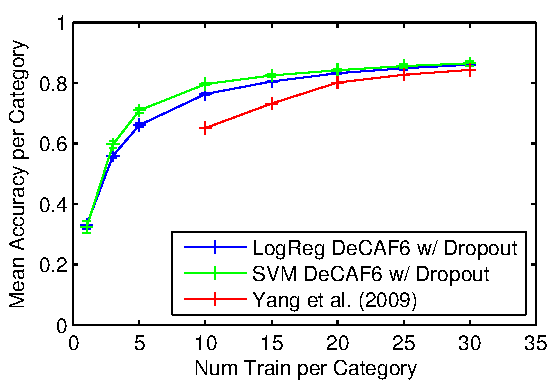
\includegraphics[width=0.5\textwidth]{figs/decaf/caltech101_plot_numtrain.pdf}
  \caption{Average accuracy per class on Caltech-101 at varying training set sizes.}\label{fig:caltech101results}
\end{figure}

Our top-performing method (based on validation accuracy) trains a linear SVM on FC$_6$ with dropout, with test set accuracy of 86.9\%.
The POOL$_5$ features perform substantially worse than either the FC$_6$ or FC$_7$ features, and hence we do not evaluate them further in this work.
The FC$_7$ features generally have accuracy about 1-2\% lower than the FC$_6$ features on this task.
The dropout regularization technique uniformly improved results by 0-2\% for each classifier/feature combination.
When trained on the deep features, the SVM and logistic regression classifiers perform roughly equally well on this task.

We compare our performance against the current state-of-the-art on this benchmark from~\cite{yang09}, a method employing a combination of 5 traditional hand-engineered image features followed by a multi-kernel based classifier.
Our top-performing method outperforms this method by 2.6\%. Note that it is likely that our features could be added to the set of hand-engineered features inside of the method of~\cite{yang09} to achieve even higher performance, but we focus here only on very simple, fast methods to demonstrate the representational strength of the features alone.
Our method also outperforms by over 20\% the two-layer convolutional network of~\cite{jarrett09}, demonstrating the importance of the depth of the network used for our feature.
Note that unlike our method, these approaches from the literature do not implicitly leverage an outside large-scale image database like ImageNet.
The performance edge of our method over these approaches demonstrates the importance of multi-task learning when performing object recognition with sparse data like that available in the Caltech-101 benchmark.

To further explore the impact of sparse training data on our method's performance, we also show how performance of the two Layer 6 + dropout methods above vary with the number of training cases per category, plotted in Figure~\ref{fig:caltech101results}. Results are again given in terms of mean accuracy per class averaged across five random data splits, and parameters in this case were kept fixed. The $i^{\mathrm{th}}$training set split at size $M$ is a subset of the $i^{\mathrm{th}}$ split at size $N$ for any $N > M$ to ensure consistency between results. Surprisingly, with just a \textit{single} labeled instance per category (one-shot learning) we are able to learn a reasonably useful classifier on the 102-category classification task, achieving accuracy of 33.0\% compared to chance accuracy of $<1$\%. This suggest that with sufficiently strong representations like the ones in this thesis, useful models of visual categories can often be learned from just a single positive example.

\subsection{Domain Adaptation}
We next evaluate the deep features for use on the task of domain adaptation. For our experiments we use the benchmark \textit{Office} dataset \cite{saenko2010adapting}.The dataset contains three domains: \texttt{Amazon}, which consists of product images taken from \url{amazon.com}; and \texttt{Webcam} and \texttt{Dslr}, which consist of images taken in an office environment using a webcam or digital SLR camera, respectively. 

In the domain adaptation setting, we are given a training (source) domain with labeled training data and a distinct test (target) domain with either a small amount of labeled data or no labeled data. We will experiment within the supervised domain adaptation setting, where there is a small amount of labeled data available from the target domain. 

Most prior work for this dataset uses SURF \cite{surf06} interest point features (available for download with the dataset). To illustrate the ability of deep features to be robust to resolution changes, we use the t-SNE~\cite{tsne} algorithm to project both SURF and FC$_6$, computed for \texttt{Webcam} and \texttt{Dslr}, into a 2D visualizable space (See Figure~\ref{fig:office_vis}). We visualize an image on the point in space corresponding to its low dimension projected feature vector. We find that the deep features not only provides better within category clustering, but also clusters same category instances across domains, effectively \emph{undoing} the domain bias, or the ``dataset bias'' as described by Torralba and Efros \cite{torralba_cvpr11}.

\newcommand{\soffice}{.3\linewidth}
\begin{figure}
\centering
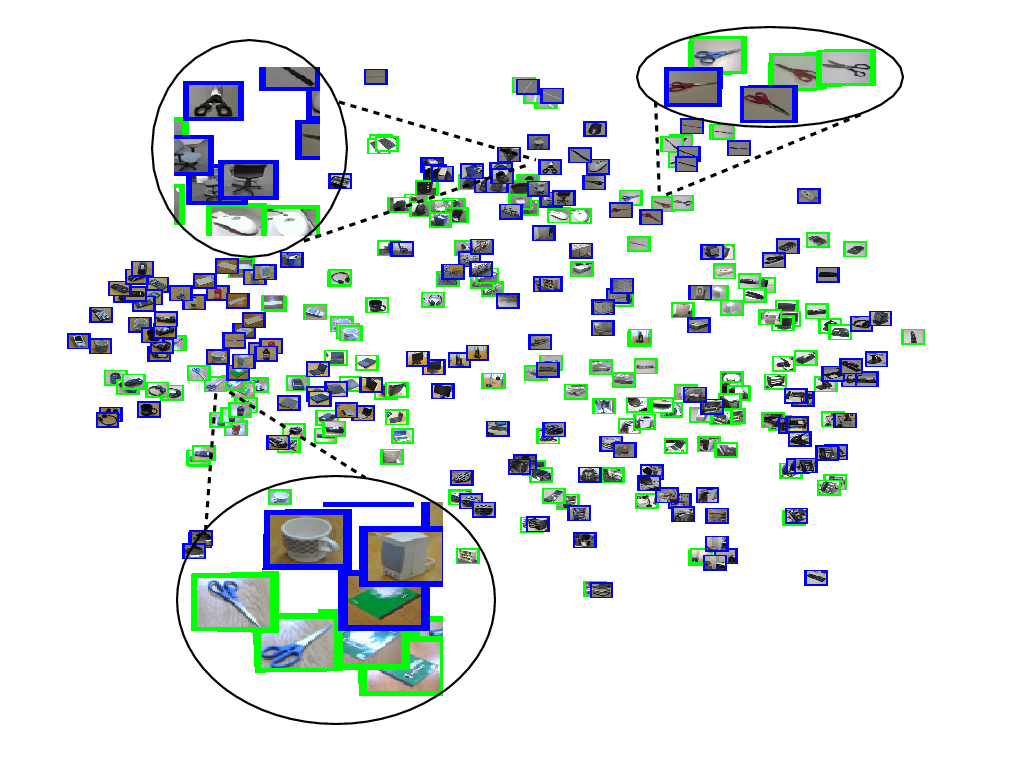
\includegraphics[height=\soffice]{figs/decaf/surf_webcam_dslr_vis_overlay.png}
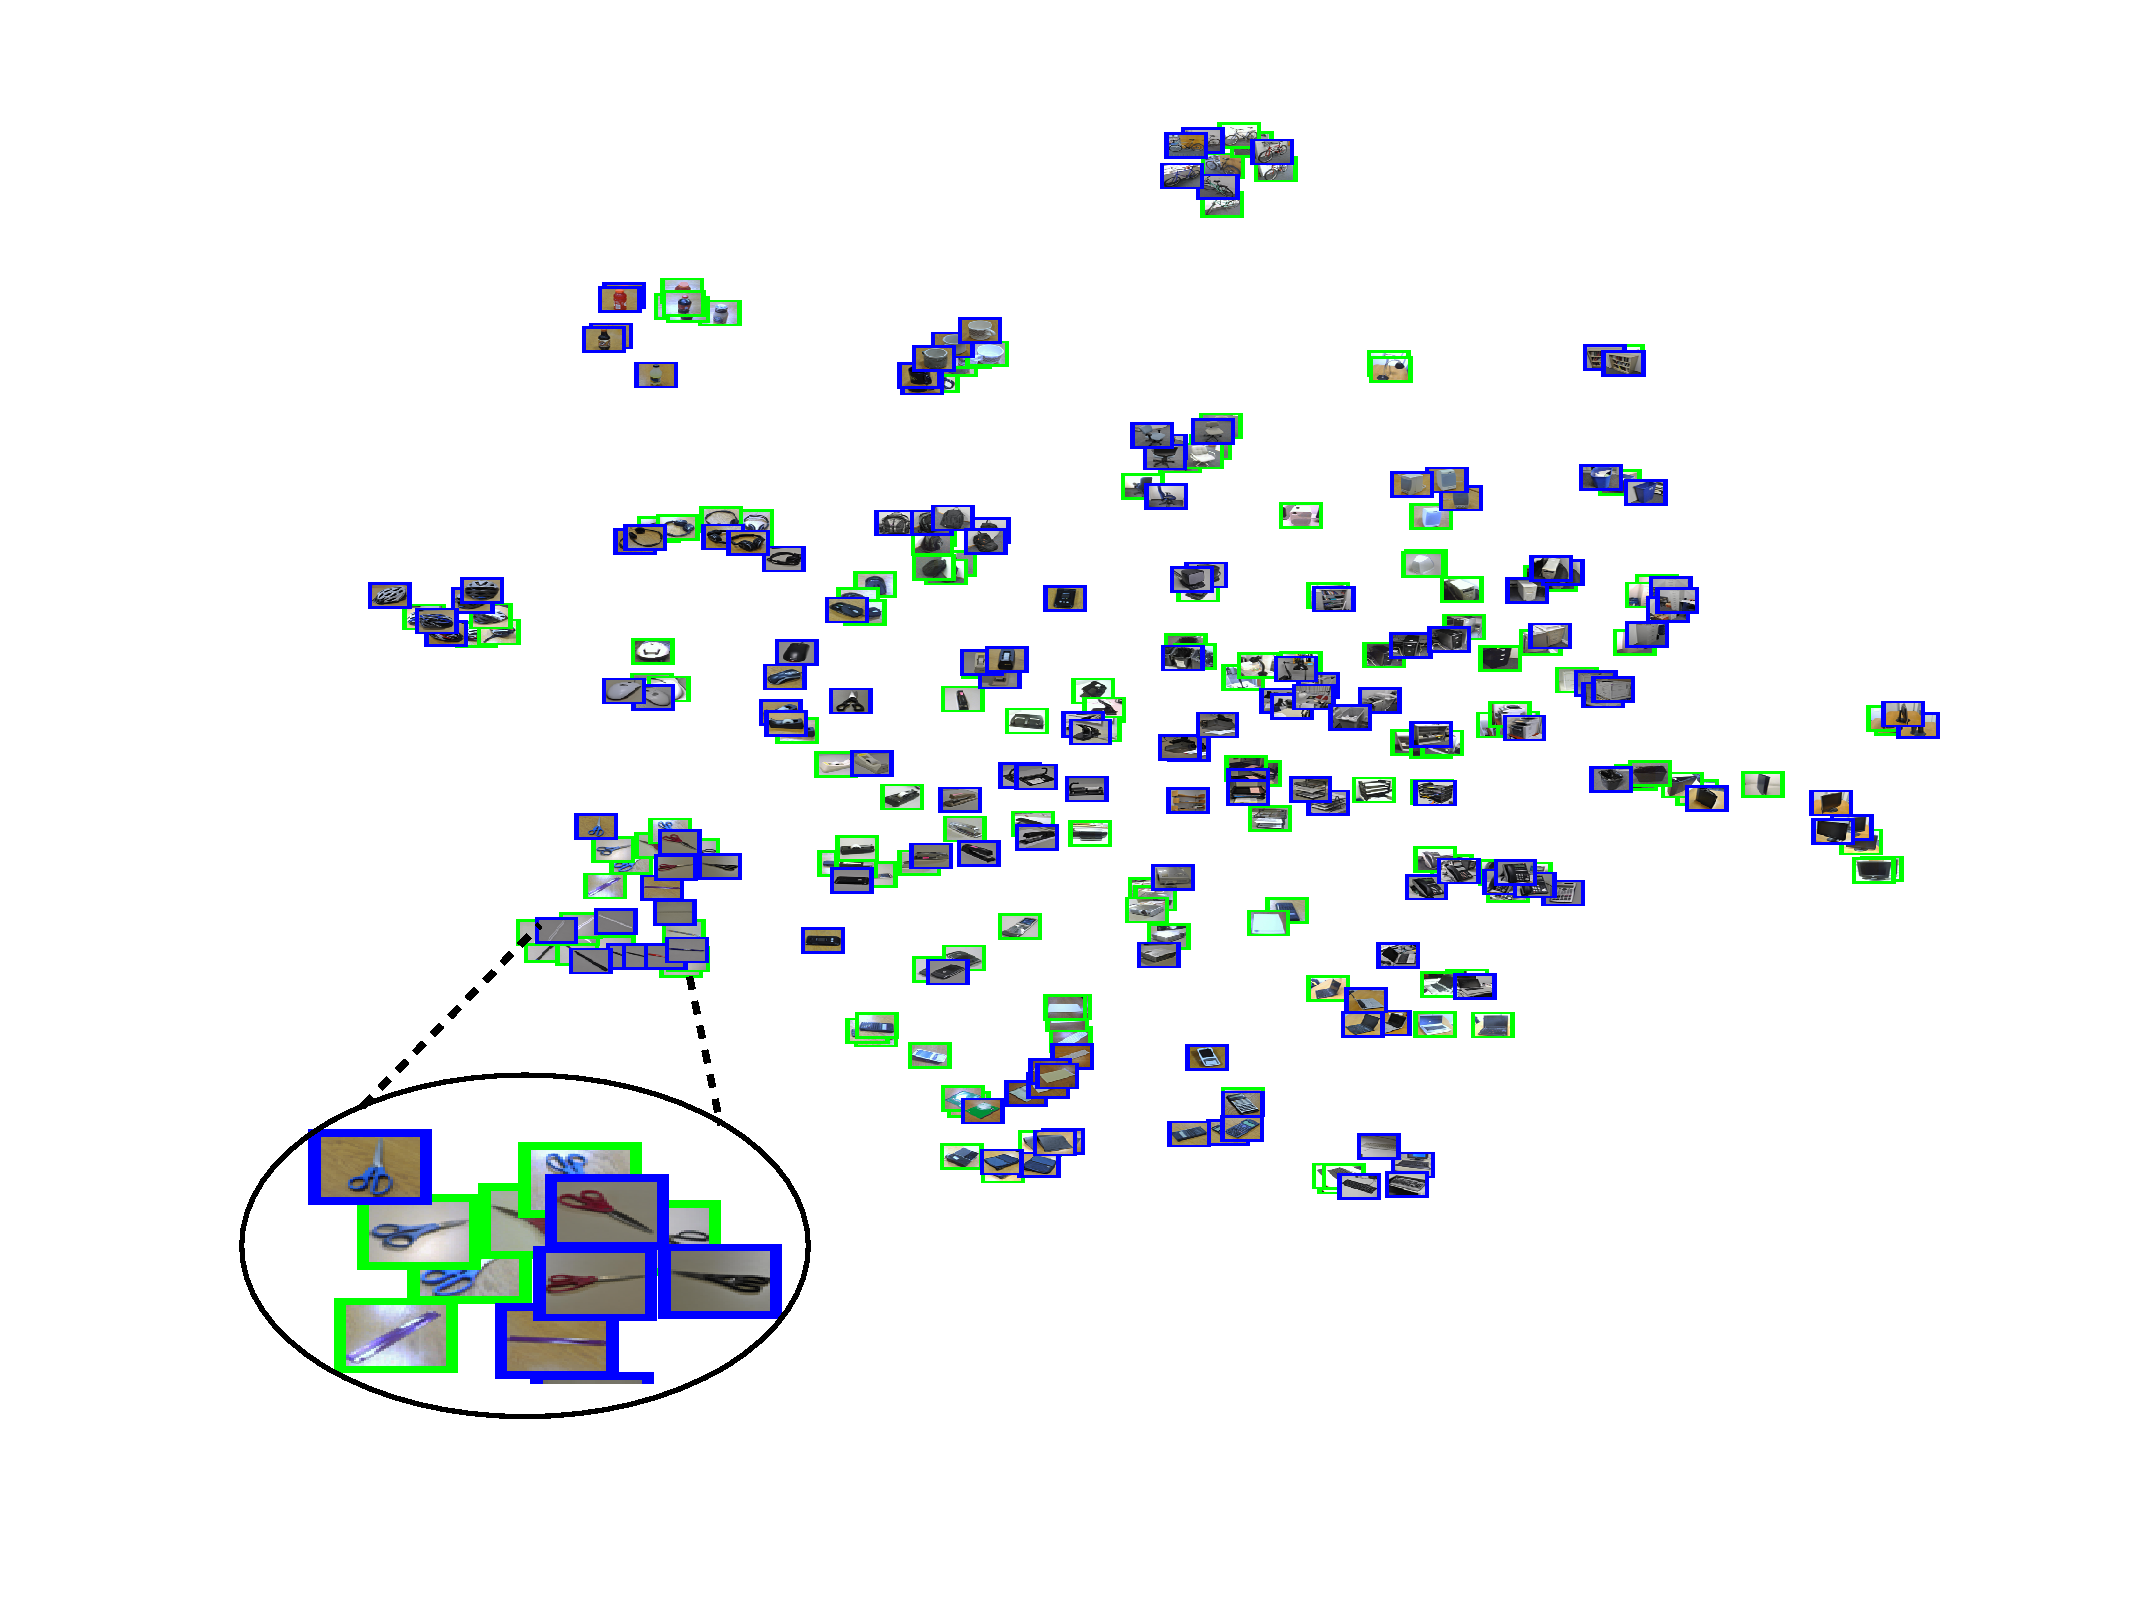
\includegraphics[height=\soffice]{figs/decaf/fc6_webcam_dslr_vis_overlay1}
\caption{Visualization of the webcam (green) and dslr (blue) domains using the original released SURF features (left) and FC$_6$ (right). The figure is best viewed by zooming in to see the images in local regions. All images from the scissor class are shown enlarged. They are well clustered and overlapping in both domains with our representation, while SURF only clusters a subset and places the others in disjoint parts of the space, closest to distinctly different categories such as chairs and mugs.}
\label{fig:office_vis}
\end{figure}

\newcommand{\ra}[1]{\renewcommand{\arraystretch}{#1}}

\begin{table}
\small
\begin{center}
\ra{1.1}
\tabcolsep=0.11cm
\begin{tabular}{@{} cccccccc @{}}
& \multicolumn{3}{c}{\texttt{Amazon} $\rightarrow$ \texttt{Webcam}} & \phantom{ab} & \multicolumn{3}{c}{\texttt{Dslr} $\rightarrow$ \texttt{Webcam}}\\
\cmidrule{2-4} \cmidrule{6-8}
	& SURF & FC$_6$ & FC$_7$  && SURF& FC$_6$ & FC$_7$\\
        	\midrule
LogReg(S) & $  9.63\pm    1.4$ & $ 48.58\pm    1.3$ & $ 53.56\pm    1.5$ && $ 24.22\pm    1.8 $ & $ 88.77\pm    1.2$ & $ 87.38\pm    2.2$ \\
SVM(S) & $ 11.05\pm    2.3$ & $ 52.22\pm    1.7$ & $ 53.90\pm    2.2$ && $ 38.80\pm    0.7 $ & $ 91.48\pm    1.5$ & $ 89.15\pm    1.7$ \\
%\\
LogReg(T) & $ 24.33\pm    2.1$ & $ 72.56\pm    2.1$ & $ 74.19\pm    2.8$ && $ 24.33\pm    2.1 $& $ 72.56\pm    2.1$ & $ 74.19\pm    2.8$ \\
SVM(T) & $ 51.05\pm    2.0$ &  $ 78.26\pm    2.6$ & $ 78.72\pm    2.3$ && $ 51.05\pm    2.0 $&  $ 78.26\pm    2.6$ & $ 78.72\pm    2.3$ \\
%\\
LogReg(ST) & $ 19.89\pm    1.7$  & $ 75.30\pm    2.0$ & $ 76.32\pm    2.0$ && $ 36.55\pm    2.2 $ & $ 92.88\pm    0.6$ & $ 91.91\pm    2.0$ \\
SVM(ST) & $ 23.19\pm    3.5$  & $ 80.66\pm    2.3$ & $ 79.12\pm    2.1$ && $ 46.32\pm    1.1 $&$\bm{ 94.79\pm    1.2}$ & $ 92.96\pm    2.0$ \\
 \\
\cite{ref:daume} & $ 40.26\pm    1.1$  & $\bm{82.14\pm    1.9}$ & $ 81.65\pm    2.4$ && $ 55.07\pm    3.0 $ & $ 91.25\pm    1.1$ & $ 89.52\pm    2.2$ \\
\cite{Hoffman13:ELD} & $ 37.66\pm    2.2$  & $ 80.06\pm    2.7$ & $ 80.37\pm    2.0$ && $ 53.65\pm    3.3 $ & $ 93.25\pm    1.5$ & $ 91.45\pm    1.5$ \\
\cite{ref:gong12_gfk} & $ 39.80\pm    2.3$ &  $ 75.21\pm    1.2$ & $ 77.55\pm    1.9$ & &$ 39.12\pm    1.3 $ & $ 88.40\pm    1.0$ & $ 88.66\pm    1.9$ \\
\cite{ref:dlid} & \multicolumn{3}{c}{58.85} && \multicolumn{3}{c} {78.21}\\
\hline
\end{tabular} 
\end{center}
\caption{Deep features dramatically outperforms the baseline SURF feature available with the \textit{Office} dataset as well as the deep adaptive method of \cite{ref:dlid}. We report average multi-class accuracy using both standard and adaptive classifiers, changing only the input feature from SURF to deep features. Surprisingly, in the case of \texttt{Dslr}$\rightarrow$\texttt{Webcam} the domain shift is largely non-existent with the new features.}
\label{tab:office}
\end{table}

We validate this conclusion with a quantitative experiment on the \textit{Office} dataset. Table \ref{tab:office} presents multi-class accuracy averaged across 5 train/test splits for the domain shifts \texttt{Amazon}$\rightarrow$\texttt{Webcam} and \texttt{Dslr} $\rightarrow$ \texttt{Webcam}. We use the standard experimental setup first presented in \cite{saenko2010adapting}. To compare SURF with the FC$_6$ and FC$_7$ features, we report the multi-class accuracy for each, using an SVM and Logistic Regression both trained in 3 ways: with only source data (S), only target data (T), and source and target data (ST). We also report results for three adaptive methods run with each deep feature we consider as input. Finally, for completeness we report a recent and competing deep domain adaptation result from \cite{ref:dlid}. It is observed that by adopting deep features alone, one could dramatically outperform the baseline SURF feature available with the \textit{Office} dataset as well as the deep adaptive method of \cite{ref:dlid}. 


\begin{figure}[t]
\centering
\begin{tabular}{ccc}
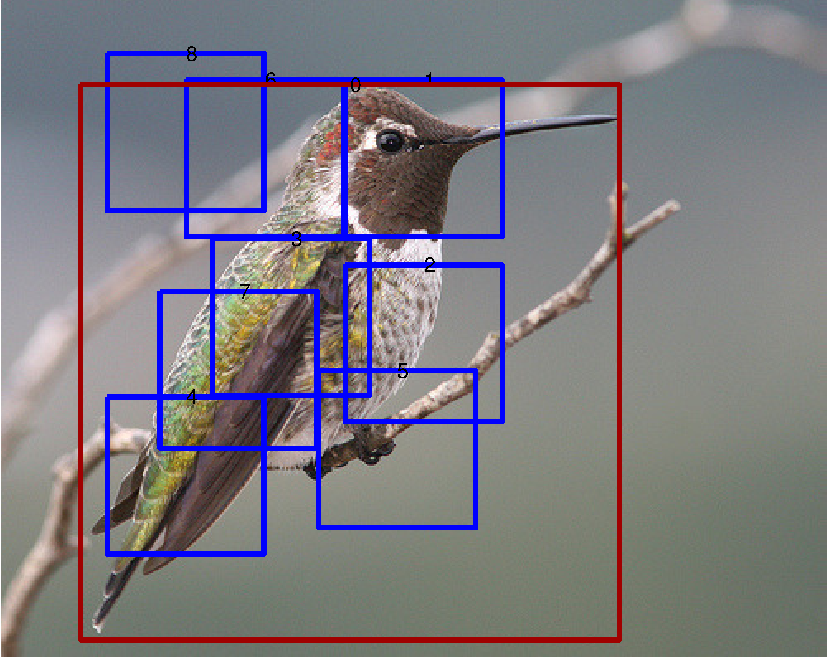
\includegraphics[height=0.3\linewidth]{figs/decaf/bird_detection} &
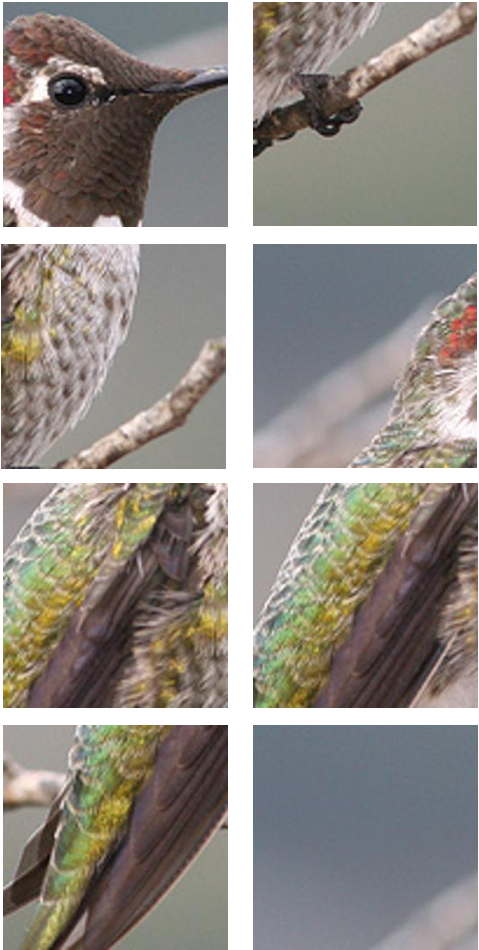
\includegraphics[height=0.3\linewidth]{figs/decaf/bird_with_parts} &
\raisebox{24mm}{\begin{minipage}{.2\linewidth}
\centering
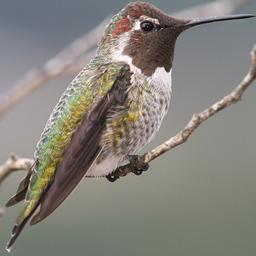
\includegraphics[height=0.47\linewidth]{figs/decaf/bbox.jpg} \\
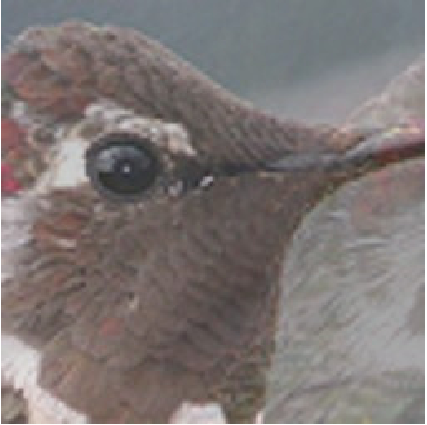
\includegraphics[height=0.47\linewidth]{figs/decaf/bird_head} \\
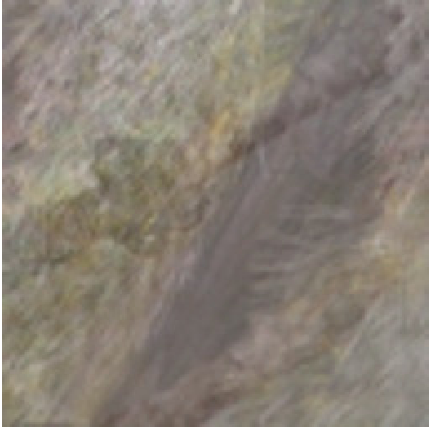
\includegraphics[height=0.47\linewidth]{figs/decaf/bird_body}
\end{minipage}}\\
DPM Detections & Parts & DPD \\
\end{tabular}
\caption{The pipeline of the deformable part descriptor (DPD) on a sample test images. It uses DPM for part localization and then uses learned pooling weights for the final pose-normalized representation.}
\label{fig:birds}
\end{figure}

\begin{table}
\centering
\begin{tabular}{lc}
\toprule
Method & Accuracy\\
\midrule
FC$_6$  & 58.75 \\
DPD + FC$_6$ & {\bfseries 64.96} \\
\\
DPD \cite{dpd}& 50.98 \\
POOF \cite{poof}& 56.78 \\
\bottomrule
\end{tabular}
\caption{Accuracy on the Caltech-UCSD bird dataset.}
\label{table:birds}
\end{table}

\subsection{Fine-Grained Recognition}
We tested the performance of deep features on the task of subcategory recognition. To this end, we adopted one of its most popular tasks - the Caltech-UCSD birds dataset~\cite{birds}, and compare the performance against several state-of-the-art baselines.

Following common practice in the literature, we adopted two approaches to perform classification. Our first approach adopts an ImageNet-like pipeline, in which we followed the existing protocol by cropping the images regions $1.5\times$ the size of the provided bounding boxes, resizing them 256$\times$256 and then feeding them into the convolutional pipeline to get the features for classification. For simplicity, we computed FC$_6$ and trained a multi-class logistic regression on top of the features.

Our second approach, we tested the deep features in a pose-normalized setting using the deformable part descriptors (DPD) method~\cite{dpd}. Inspired by the deformable parts model \cite{dpm}, DPD explicitly utilizes the part localization to do semantic pooling. Specifically, after training a weakly-supervised DPM on bird images, the pool weight for each part of each component is calculated by using the key-point annotations to get cross-component semantic part correspondence. The final pose-normalized representation is computed by pooling the image features of predicted part boxes using the pooling weights. Based on the DPD implementation provided by the authors, we applied deep feature extraction in the same pre-trained DPM model and part predictions and used the same pooling weights. Figure \ref{fig:birds} shows the DPM detections and visualization of pooled DPD features on a sample test image.  As our first approach, we resized each predicted part box to 256 $\times$ 256 and computed FC$_6$ to replace the KDES image features \cite{kdes} used in the original DPD paper \cite{dpd}.

Our performance as well as those from the literature are listed in Table \ref{table:birds}. Deep features together with a simple logistic regression already obtains a significant performance increase over existing approaches, indicating that such features, although not specifically designed to model subcategory-level differences, captures such information well. In addition, explicitly taking more structured information such as part locations still helps, and provides another significant performance increase, obtaining an accuracy of 64.96\%, compared to the 50.98\% accuracy reported in~\cite{dpd}. It also outperforms POOF \cite{poof}, to our knowledge the best accuracy reported in the literature prior to this work.

We note again that in all the experiments above, no fine-tuning is carried out on the lower-level layers, since our main interest is to analyze how well a feature extraction pipeline trained with a different objective generalizes to different tasks. To obtain the best possible result one may want to perform a full back-propagation, as have been shown effective in specific applications like detection \cite{girshick2013rich}. However, the fact
that we see a significant performance increase without fine-tuning suggests that
a pre-trained deep network may already serve as a good off-the-shelf visual representation without heavy computation.

\subsection{Scene Recognition}
Finally, we evaluate the deep features on the scene recognition benchmarks, namely the SUN-397 large-scale scene recognition database~\cite{xiao10}. Unlike object recognition, wherein the goal is to identify and classify an object which is usually the primary focus of the image, the goal of a scene recognition task is to classify the \textit{scene} of the entire image.
In the SUN-397 database, there are 397 semantic scene categories including \textit{abbey}, \textit{diner}, \textit{mosque}, and \textit{stadium}.
Because the Caffe features are learned on ILSVRC, an object recognition database, we are applying it to a task for which it was not designed.
Hence we might expect this task to be very challenging for these features, unless they are highly generic representations of the visual world.

Based on the success of using dropout with FC$_6$ and FC$_7$ for the object recognition task detailed in Section~\ref{sec:caltech}, we train and evaluate linear classifiers on these dropped-out features on the SUN-397 database.
Table~\ref{tab:sunresults} gives the classification accuracy results averaged across 5 splits of 50 training images and 50 test images.
Parameters are fixed for all methods, but we select the top-performing method by cross-validation, training on 42 images and testing on the remaining 8 in each split.

Our top-performing method in terms of cross-validation accuracy was to use FC$_7$ with the SVM classifier, resulting in 40.94\% test performance.
Comparing against the method of~\cite{xiao10}, the current state-of-the-art method, we see a performance improvement of 2.9\% using the feature off-the-shelf and without any ensembles with additional features.
Note that, like the state-of-the-art method used as a baseline in Section~\ref{sec:caltech}, this method uses a large set of traditional vision features and combines them with a multi-kernel learning method.
The fact that a simple linear classifier on top of our single image feature outperforms the multi-kernel learning baseline built on top of many traditional features demonstrates the ability of deep features to generalize to other tasks and its representational power as compared to traditional hand-engineered features.

\begin{table}
\centering
\begin{tabular}{lcc}%{|c|c|c|}
\hline
& FC$_6$ & FC$_7$ \\
\hline
LogReg & $\bm{ 40.94 \pm 0.3}$ & $40.84 \pm 0.3$ \\
SVM & $39.36 \pm 0.3$ & $40.66 \pm 0.3$ \\
\hline
Xiao \etal \cite{xiao10} & \multicolumn{2}{c}{38.0} \\
\hline
\end{tabular}
\caption{Average accuracy per class on SUN-397 with 50 training samples and 50 test samples per class, across two hidden layers of the network and two classifiers. Note that the result from the training protocol/classifier combination with the best validation accuracy is FC$_7$, while FC$_6$ has the best testing accuracy. However the difference between them is not statistically significant.}
\label{tab:sunresults}
\end{table}

\section{Emergence of Conceptual Embeddings}
In addition to quantitatively analyze the learned features by stacking a classifier on top of them, an alternate way to qualitatively show the effectiveness of various features is to look at their distribution in the feature space with respect to high-level semantics, such as object labels. To this end, we will visualized the model features to gain insight into the semantic capacity of the various features that have been typically employed in computer vision. In particular, we compare the learned deep features with GIST features \cite{gist} and LLC features \cite{llc}.

The features in the following way: we run the t-SNE algorithm \cite{tsne} to find a 2-dimensional embedding of the high-dimensional feature space, and plot them as points colored depending on their semantic category in a particular hierarchy. We did this on the validation set of ILSVRC-2012 to avoid overfitting effects (as the deep CNN used in this paper was trained only on the training set), and also use an independent dataset, SUN-397 \cite{xiao10}, to evaluate how dataset bias affects our results (see e.g. \cite{torralba_cvpr11} for a deeper discussion of this topic). For high-dimensional features such as LLC, we first generate a random orthonormal matrix and perform dimensionality reduction to obtain a 512-dimensional feature space. It is known from the Johnson–Lindenstrauss lemma that such random projection preserves Euclidean distance to a satisfying granularity, thus not hurting the final embedding result.


\newcommand{\fsize}{.45\linewidth}
\begin{figure}
  \begin{tabular}{cc}
    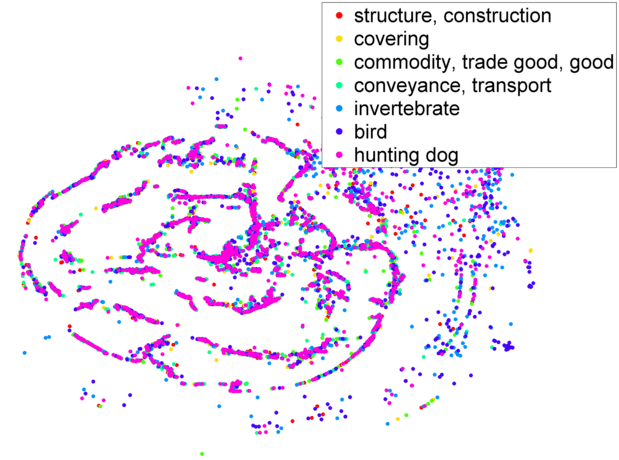
\includegraphics[width=\fsize]{figs/decaf/LLC_quarter-fs8.png} & 
    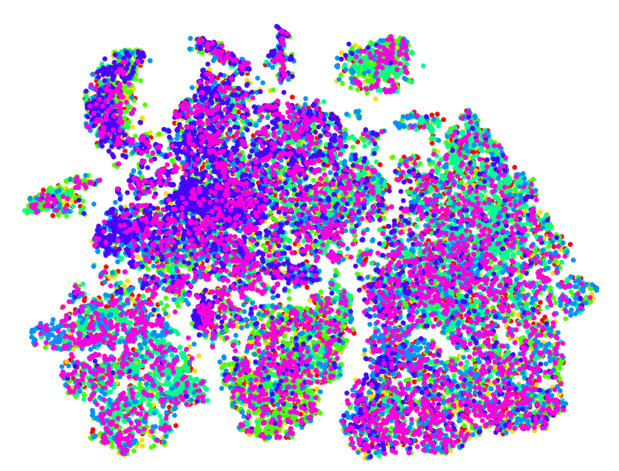
\includegraphics[width=\fsize]{figs/decaf/gist_quarter-fs8.png}\\
    (a) LLC & (b) GIST \\
    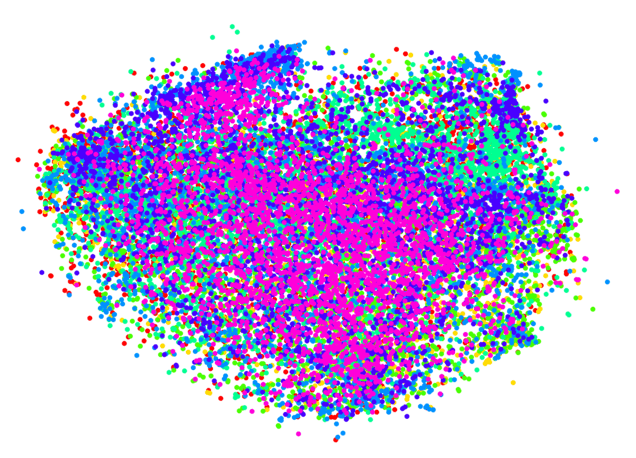
\includegraphics[width=\fsize]{figs/decaf/pool1_quarter-fs8.png} & 
    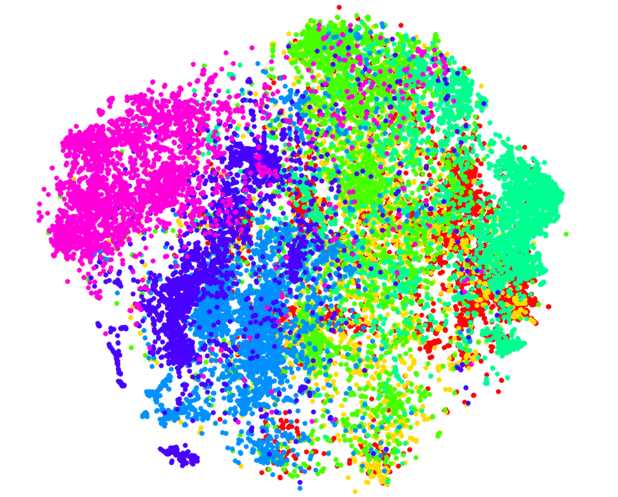
\includegraphics[width=\fsize]{figs/decaf/fc6_quarter-fs8.png} \\
    (c) POOL$_1$ & (d) FC$_6$\\
  \end{tabular}
  \caption{This figure shows several t-SNE feature visualizations on the ILSVRC-2012 validation set. (a) LLC , (b) GIST, and features derived from our CNN: (c) POOL$_1$, the first pooling layer, and (d) FC$_6$, the second to last hidden layer. The figure is best viewed in color. \label{fig:embedding}}
\end{figure}

We first visualize the semantic segregation of the model by plotting
the embedding of labels for higher levels of the WordNet hierarchy;
for example, a strong feature for visual recognition should cluster
animals and non-animals instances separately, even though there is no
explicit modeling through the supervised training of the CNN\footnote{We note that during training, labels are considered flat, \ie ``cat'' is as negative as ``car'' for a dog image. Thus, the semantic segregation of high-level clusters should be interpreted as emerging from data, not supervised information.}.
 Figure~\ref{fig:embedding} shows the features extracted on the validation set using the first pooling layer, and the second to last hidden layer FC$_6$, showing a clear semantic clustering in the latter but not in the former. This is compatible with common deep learning knowledge that the first layers learn ``low-level'' features, whereas the latter layers learn semantic or ``high-level'' features.
 
Furthermore, baseline features such as GIST or LLC fail to capture the semantic difference in the image (although they show interesting clustering structure). For GIST, it focuses more on holistic layouts of the objects, but does not take into account specific label information. For LLC, the embedding is highly sparse, possibly due to the fact that LLC is a highly over-complete feature designed to work well with linear kernels, effectively pulling all data points far from each other.


More interestingly, we note that such semantic segregation is, at least to some extent, transferrable to related but different datasets. In Figure~\ref{fig:generalization} we visualize the top performing features (DeCAF$_6$) on the SUN-397 dataset, also embedded with t-SNE in a two dimensional space. Although the features are never trained to distinguish scenes and have not seen such labels, they show very good clustering of semantic classes (e.g., indoor vs. outdoor). This suggests that intermediate layer outputs serve as good features for general object recognition tasks, considering the case where the object class that we are trying to detect is not in the original object pool of ILSVRC-2012.

\begin{figure}
\centering
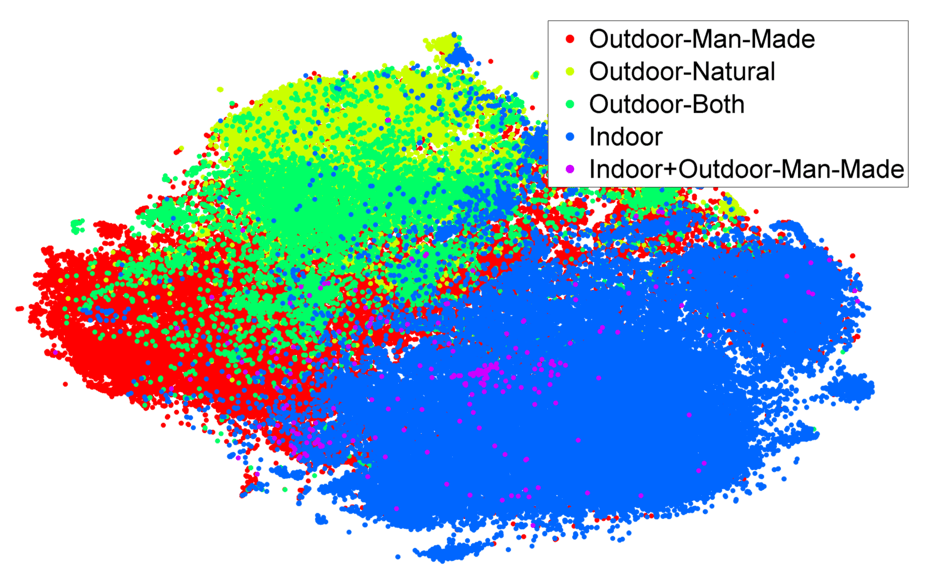
\includegraphics[width=.6\linewidth]{figs/decaf/SUN397_quarter-fs8.png}
\caption{In this figure we show how our features trained on ILSVRC-2012 generalized to SUN-397 when considering semantic groupings of labels. Best viewed in color. \label{fig:generalization}}
\end{figure}

\subsection{Perceptual Embedding of Visual Concepts: A Conjecture}

It is worth noting that the natural emergence of concept-level grouping is closely related to the concept learning framework I proposed in the previous chapter. Specifically, existing concept learning frameworks requires a pre-designed hierarchy, which defines the ``closeness'' between various object categories in a conceptual space, to be provided as oracle knowledge. While this is available in specific use cases such as WordNet, it is nonetheless complete, and determining the correct conceptual hierarchy is an open problem yet to be explored.

With the intermediate features from a deep model, here I present a conjecture that grounds semantics directly in the \emph{perceptual} space obtained from dee features, rather than a separate label hierarchy that is manually constructed. Specifically, one could view the distance in the embedded space as a measure of semantic closeness. For example, for an image of dalmatian, closest to it will be other related dalmatians; further in the space would be other breeds of dogs, other animals, and finally non-animal images. Two possible directions would naturally follow:

\paragraph{Learning Nested Embeddings} What has been shown in the previous section is the natural emergence of conceptual hierarchy in the flat learning procedure. While this has already been performing well qualitatively, a natural choice to learn a better embedding space is to utilize the hierarchy that ImageNet/WordNet provides. Specifically, one would be able to learn a better embedding with what could be called ``nested distance metric learning'': for a triplet of images such as a dalmatian, a corgi and a tabby cat, one can enforce relative comparison constraints \cite{schultz2003learning}.

\paragraph{Learning Concept Prior} With the learned embedded space, one could construct concept priors and conditionals in the perceptual space following the similar ideas we use for the conceptual space. One possible concept definition that is most likely to succeed is to define concepts as Gaussian distributions\footnote{I propose Gaussian distribution to provide some level of continuity, although one could certainly binarize the probability to obtain 0-1 predictions.} in the perceptual space, with the standard deviation of the distribution serving as the ``width'' of the concept: for example, ``dog'' would have a larger width than ``dalmatian''. The prior of such concepts could then be constructed on top of the mean and the variance of such gaussian distributions, and a mathematically convenient choice would be a Wishart distribution, leading to a conjugate prior-conditional pair.

Interestingly enough, a very similar idea has been proposed by Fei-Fei \etal \cite{fei2006one}, although it was only proposed and evaluated in a limited fashion on the Caltech-101 dataset with conventional, hand-crafted features. A more detailed mathematical analysis as well as large-scale behavioral experiments will be one of my research directions in the future.

\section{Summary}
This chapter serves as the most exploratory chapter of the whole thesis: I presented Caffe, the open-source deep learning library that allows various research and applications to be built upon. Based on it, I have presented extensive analysis on how such deep features behave in various tasks, and propose possible direction towards the main topic of this thesis - to eventually learn a perceptual embedded space for concept hierarchies.



\section*{Notes}
Parts of this chapter have appeared in peer-reviewed publications as we list below:
\begin{enumerate}
\item Jeff Donahue, Yangqing Jia, Oriol Vinyals, Judy Hoffman, Ning Zhang, Eric Tzeng, Trevor Darrell. DeCAF: A Deep Convolutional Activation Feature for Generic Visual Recognition. ICML 2014.
\end{enumerate}
The Caffe package and its documentations could be found at \url{http://caffe.berkeleyvision.org/}.